\subsection*{Wyjaśnialność: Grad-CAM i mapy saliency}
Dla obrazów cechami są piksele, więc zamiast ważności cech (SHAP, permutation importance)
zastosowano metodę dedykowaną sieciom konwolucyjnym: \textbf{Grad-CAM} (wykład~5). Implementacja
własna na hookach PyTorch (\texttt{src/gradcam.py}):
\begin{enumerate}
\item zapamiętujemy aktywacje $A^k$ ostatniej warstwy konwolucyjnej (dla ResNet50: \texttt{layer4},
  2048 kanałów 7$\times$7) i gradient wyniku klasy $c$ względem nich,
\item waga kanału $\alpha_k^c$ to średni gradient w kanale $k$,
\item mapa $L^c = \mathrm{ReLU}\big(\sum_k \alpha_k^c A^k\big)$ jest skalowana do 224$\times$224
  i nakładana na obraz.
\end{enumerate}

\begin{figure}[H]
\centering
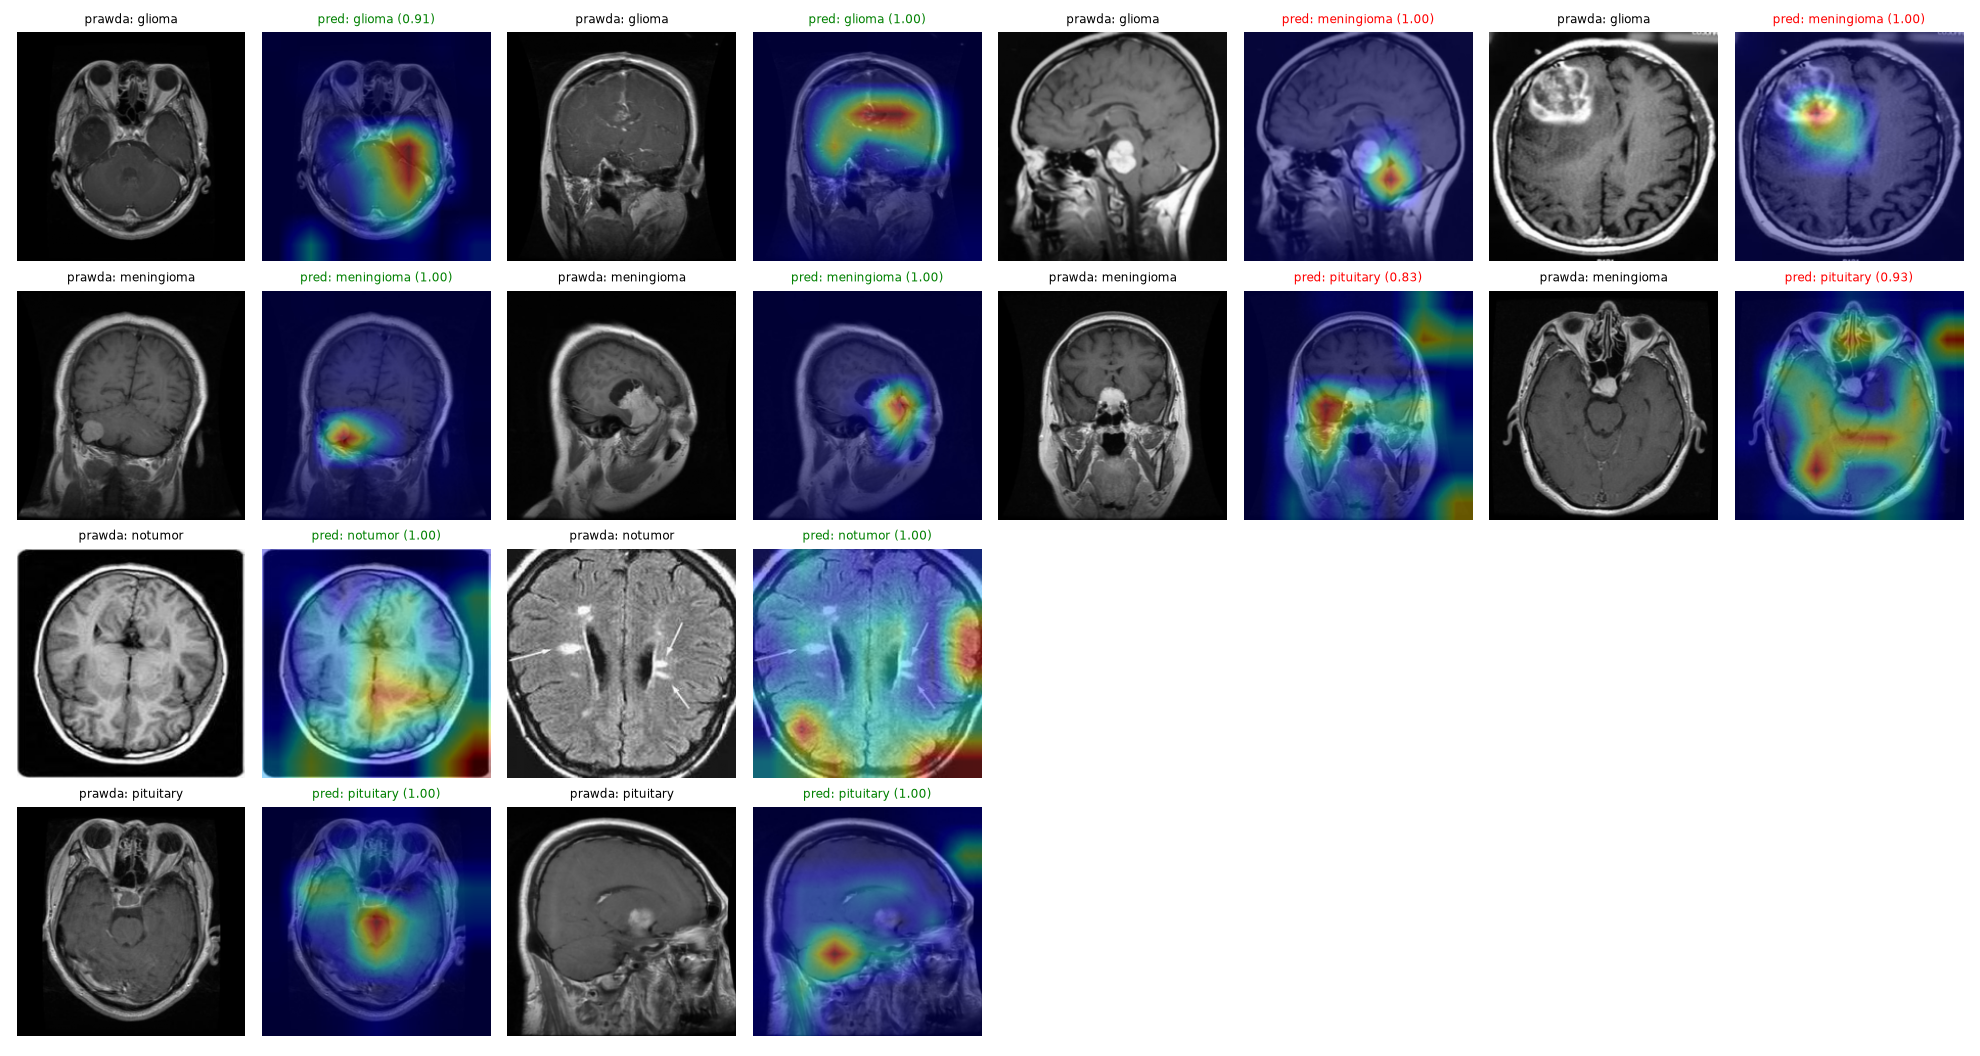
\includegraphics[width=\linewidth]{gradcam_galeria.png}
\caption{Grad-CAM dla trafnych (zielone) i błędnych (czerwone) predykcji z każdej klasy
(\texttt{test\_dedup}). Dla \texttt{notumor} i \texttt{pituitary} nie ma błędów.}
\label{fig:gradcam}
\end{figure}

Dla glejaków, oponiaków i guzów przysadki mapy w większości przypadków wskazują zmianę
nowotworową lub okolicę siodła tureckiego, czyli obszary zgodne z intuicją kliniczną
(rys.~\ref{fig:gradcam}). Dla klasy \texttt{notumor} mapa jest rozlana po całym obrazie,
także na tło i brzegi kadru. Model nie ,,sprawdza'', czy guza brak, tylko rozpoznaje ogólny
wygląd obrazu. Żeby nie opierać się na kilku wybranych obrazach (ryzyko nadinterpretacji,
wykład~5), policzono dla wszystkich obrazów \texttt{test\_dedup}, jaka część mapy leży na tle
(piksele ciemniejsze niż 20) i w pasie brzegowym (zewnętrzne 10\,\% szerokości, czyli
\borderArea{} powierzchni) -- tab.~\ref{tab:gradcam}. Dla klas z guzem na tło przypada średnio
\camBgTumor{} masy mapy, a dla \texttt{notumor} \camBgNotumor{}; na brzeg odpowiednio
\camBorderTumor{} i \camBorderNotumor{}. Mapy dla klas z guzem są więc skupione na głowie,
a dla \texttt{notumor} bliższe rozkładowi równomiernemu.

\begin{table}[H]
\centering
\caption{Gdzie leży masa mapy Grad-CAM (średnia po obrazach \texttt{test\_dedup}).}
\label{tab:gradcam}
\tabela{gradcam}
\end{table}

Dla porównania policzono najprostszą mapę saliency (moduł gradientu wyniku po pikselach,
rys.~\ref{fig:saliency}). Dla klas z guzem wskazuje podobne obszary jak Grad-CAM, ale jest
dużo bardziej zaszumiona. Dla obrazu \texttt{notumor} wyraźnie podkreśla ramkę i krawędzie
kadru, co wspiera hipotezę, że cechy techniczne obrazu (kadrowanie, źródło) wpływają na
decyzję. Metody nie są w pełni zgodne (wykład~5: niekonsekwencje technik wyjaśnialności),
a obie pokazują korelację, nie przyczynę. Traktujemy je jako wskazówkę do analizy błędów,
nie jako dowód poprawnego rozumowania modelu.

\begin{figure}[H]
\centering
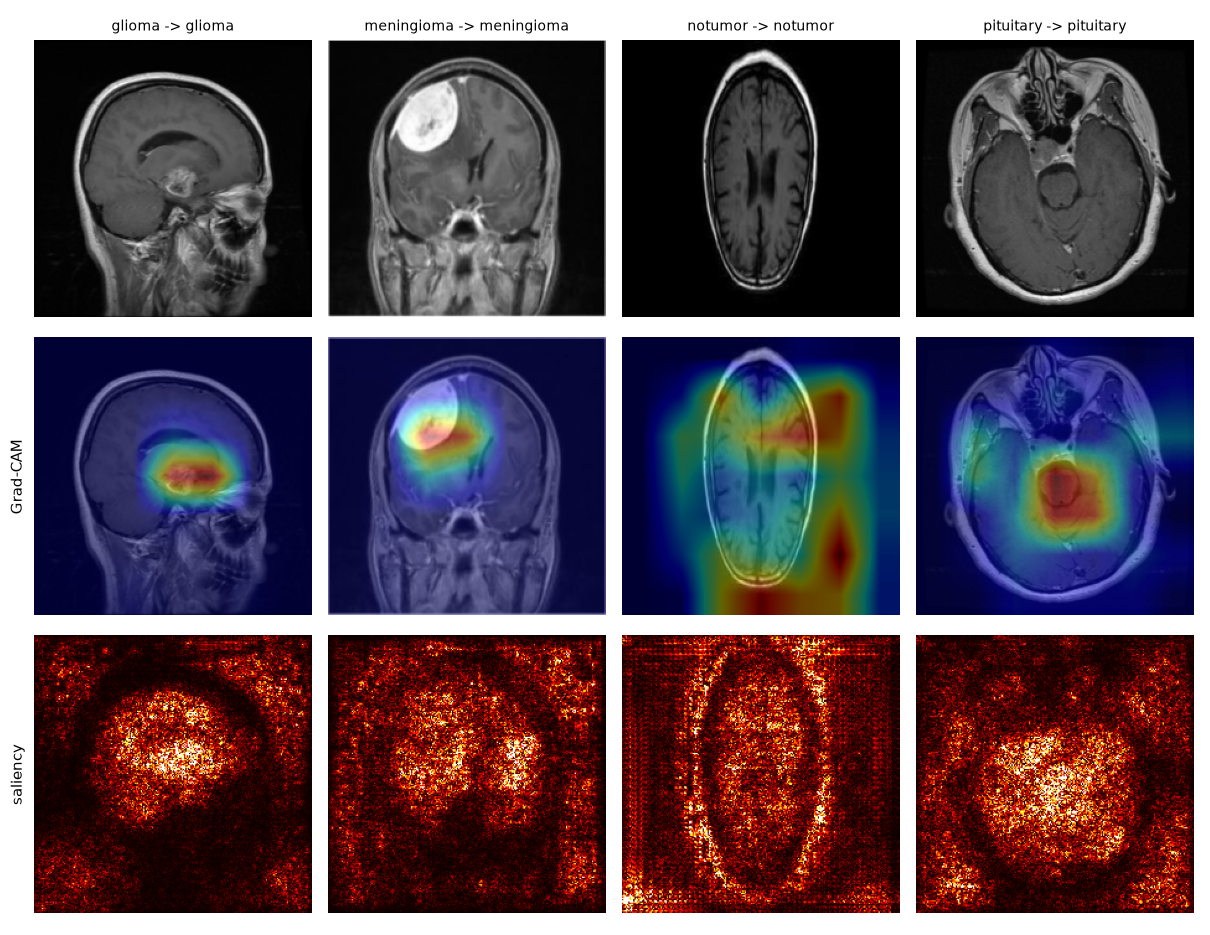
\includegraphics[width=0.75\linewidth]{gradcam_vs_saliency.png}
\caption{Ten sam obraz: Grad-CAM (środek) i mapa saliency (dół).}
\label{fig:saliency}
\end{figure}

\subsection*{Analiza błędów}\label{sec:bledy}
Najlepszy model pomylił się na \nErrTest{} z \nTestDir{} obrazów testowych, z czego
\nErrDedup{} błędów jest w \texttt{test\_dedup} (tab.~\ref{tab:bledy}). Wnioski:

\begin{table}[H]
\centering
\caption{Błędy najlepszego modelu na teście oryginalnym.}
\label{tab:bledy}
\tabela{bledy}
\end{table}

\begin{enumerate}
\item \textbf{Wyciek zawyża wynik oryginalnego testu.} Wśród obrazów, które mają w treningu
  bliźniaka tej samej klasy, odsetek błędów wynosi \errRateTwin{}, a wśród obrazów bez
  bliźniaka \errRateNoTwin{}. Dwa błędy spoza \texttt{test\_dedup} to glejaki, których
  niemal identyczny bliźniak w treningu ma etykietę \emph{oponiak}. Model ,,poprawnie
  zapamiętał'' błędną etykietę (szum etykiet z rozdz.~\ref{sec:dup}).
\item \textbf{Prawie wszystkie błędy to glejaki} (\nErrGlioma{} z \nErrTest{}):
  \nErrGliomaMeningioma{} rozpoznano jako oponiaka, a \nErrGliomaNotumor{} jako brak guza.
  Te drugie to przeoczony guz.
\item \textbf{Główna przyczyna to inne źródło obrazów (shortcut learning).} W treningu
  \emph{wszystkie} glejaki mają rozmiar 512$\times$512 (zbiór figshare, T1 po kontraście):
  glejaków o innym rozmiarze jest \gliomaOtherTrain{}. W teście jest ich \gliomaOtherTest{}
  -- pochodzą z innego źródła i często są w sekwencjach T2/FLAIR -- i model myli się na
  \gliomaOtherErr{} z nich (\gliomaOtherErrRate{}). Wśród glejaków 512$\times$512 myli się na
  \gliomaFiveErr{} z \gliomaFiveTest{}. Obrazy spoza figshare w treningu to głównie
  \texttt{notumor} (\notumorOtherTrain{}) i część oponiaków (\meningiomaOtherTrain{}), więc
  ,,nietypowy'' glejak trafia właśnie do tych klas. Model powiązał klasę ze źródłem
  i sekwencją obrazu. Przed tym ostrzegała EDA (rozdzielczość, jasność). To wyjaśnia też
  różnicę między CV a testem: w treningu nie było takich glejaków, więc walidacja krzyżowa
  nie mogła tego wykryć.
\item \textbf{Pewność nie ostrzega przed błędem.} Najbardziej pewne błędy
  (rys.~\ref{fig:bledy}) mają prawdopodobieństwo ok.~1,00. Grad-CAM pokazuje, że model
  często patrzy na sam guz, ale nadaje mu zły typ: widzi zmianę, a typ ocenia na podstawie
  wyglądu całego obrazu.
\item \textbf{Glejak a oponiak} (rys.~\ref{fig:gm}) to też para trudna z natury: oba guzy
  na pojedynczym przekroju 2D bywają podobne (wzmocnienie kontrastowe, efekt masy), a różnią
  się głównie położeniem względem opon i kształtem.
\end{enumerate}

\begin{figure}[H]
\centering
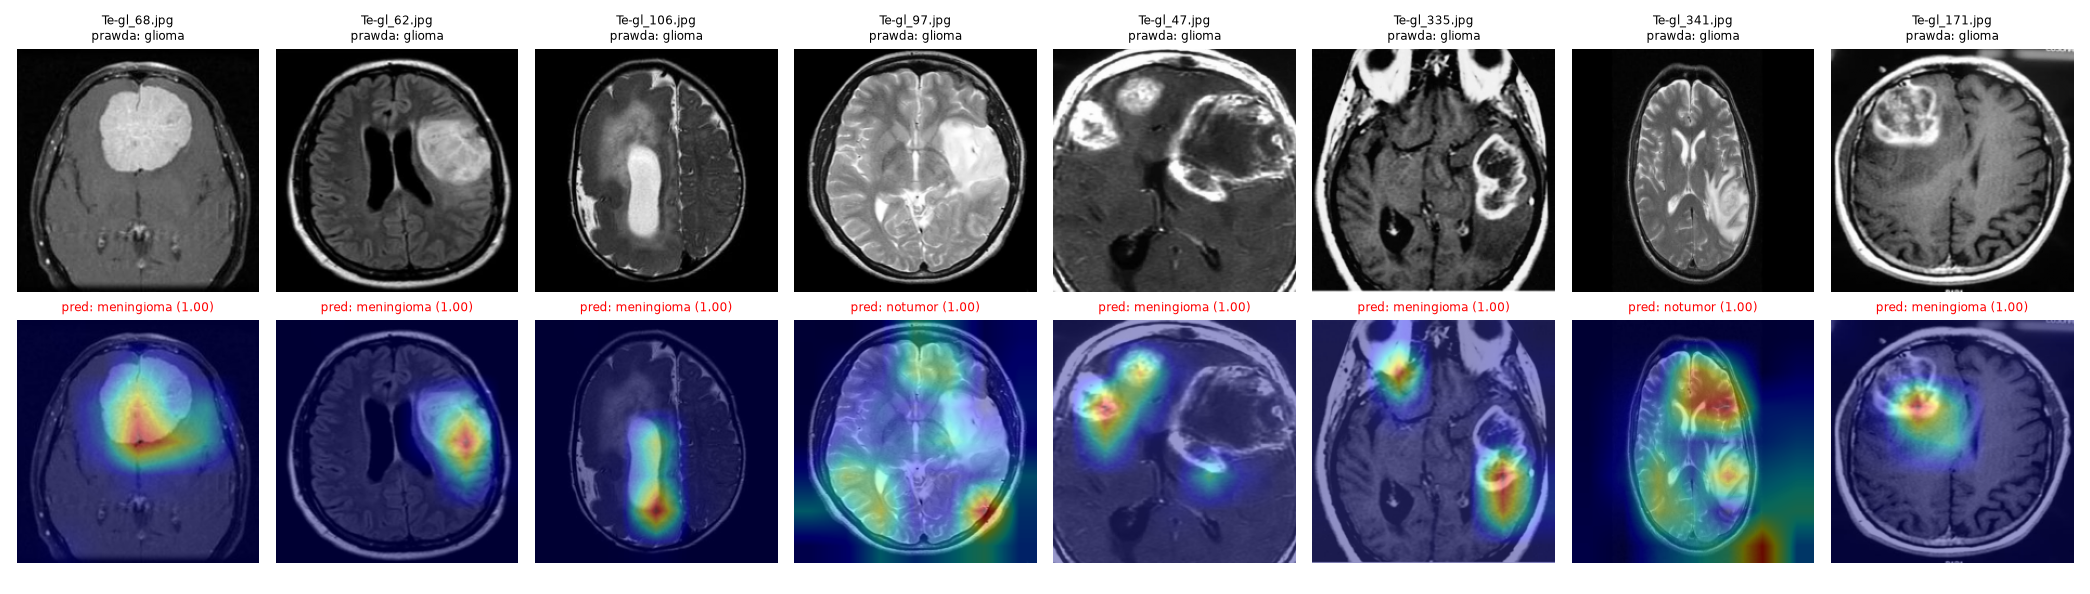
\includegraphics[width=\linewidth]{bledy_pewne.png}
\caption{Osiem najbardziej pewnych błędów najlepszego modelu z mapami Grad-CAM.}
\label{fig:bledy}
\end{figure}

\begin{figure}[H]
\centering
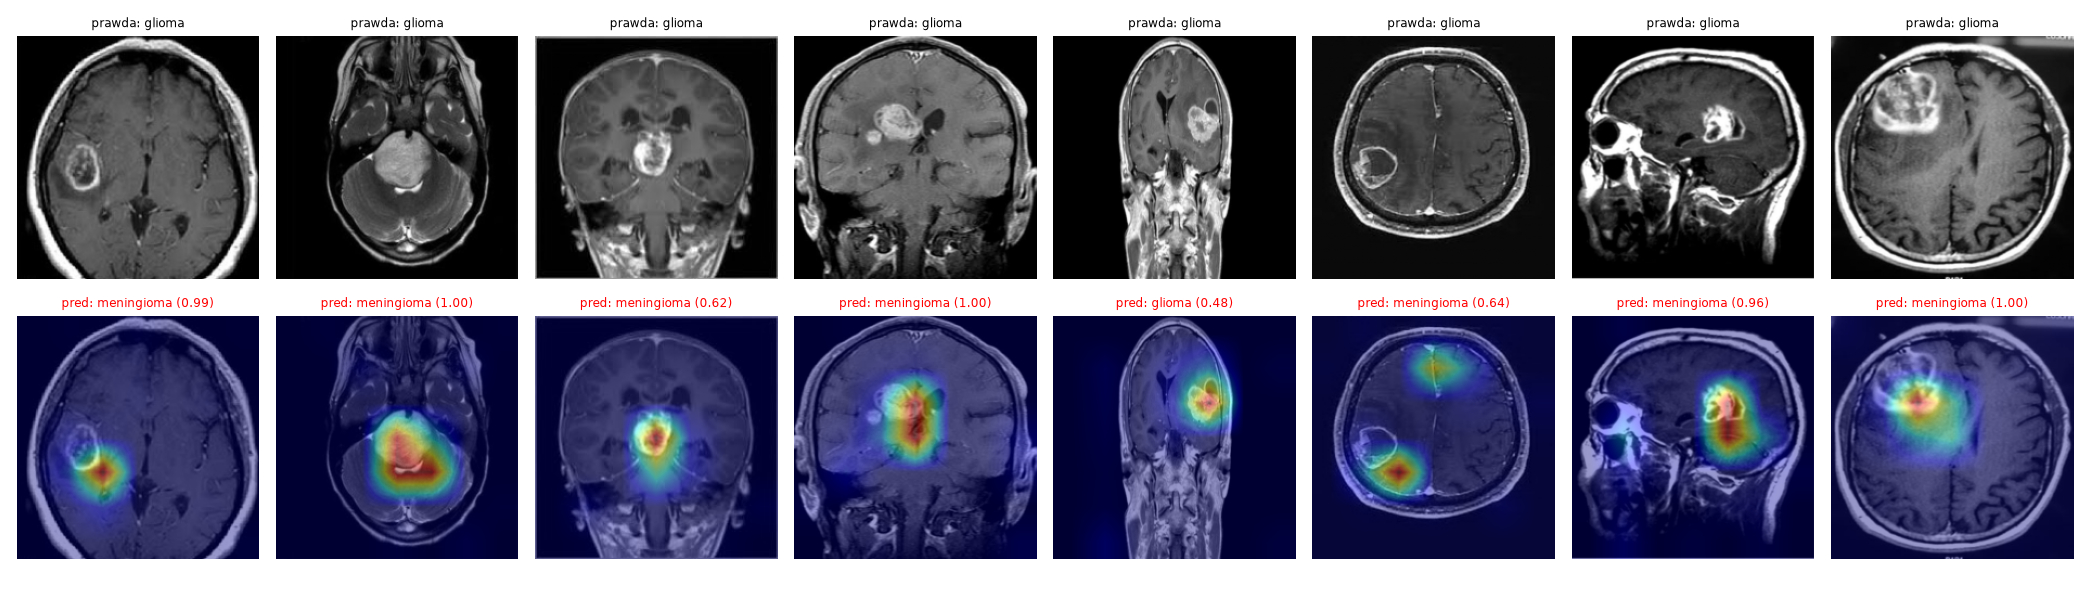
\includegraphics[width=\linewidth]{bledy_glioma_meningioma.png}
\caption{Losowe błędy glejak $\rightarrow$ oponiak.}
\label{fig:gm}
\end{figure}
